\title{Project title}
\renewcommand{\thefootnote}{\fnsymbol{footnote}}
\author{Yangkang Chen
\thanks{Y. Chen is with School of Earth Sciences, Zhejiang University, Hangzhou, Zhejiang Province, China, 310027, yangkang.chen@zju.edu.cn}
\thanks{The research is supported by the starting fund from Zhejiang University and ``Thousand Youth Talents Plan of China''.}}
\maketitle

\begin{abstract}
A brief summary of the work \cite{yangkang20142}.
\end{abstract}

\begin{keywords}
key1,key2,key3
\end{keywords}

\section{Introduction}
\section{Theory}
\section{Examples}
\section{Discussions}
\section{Conclusions}
\section{Acknowledgements}



\bibliographystyle{IEEEtran}
\bibliography{projname}



%\begin{figure}[htb!]
%	\centering
%	\subfigure[]{\includegraphics[width=0.8\textwidth]{Fig/fig}}
%	\caption{Caption.}
%	\label{fig:fig}
%\end{figure}


%\begin{figure}[htb!]
%	\centering
%	\subfigure[]{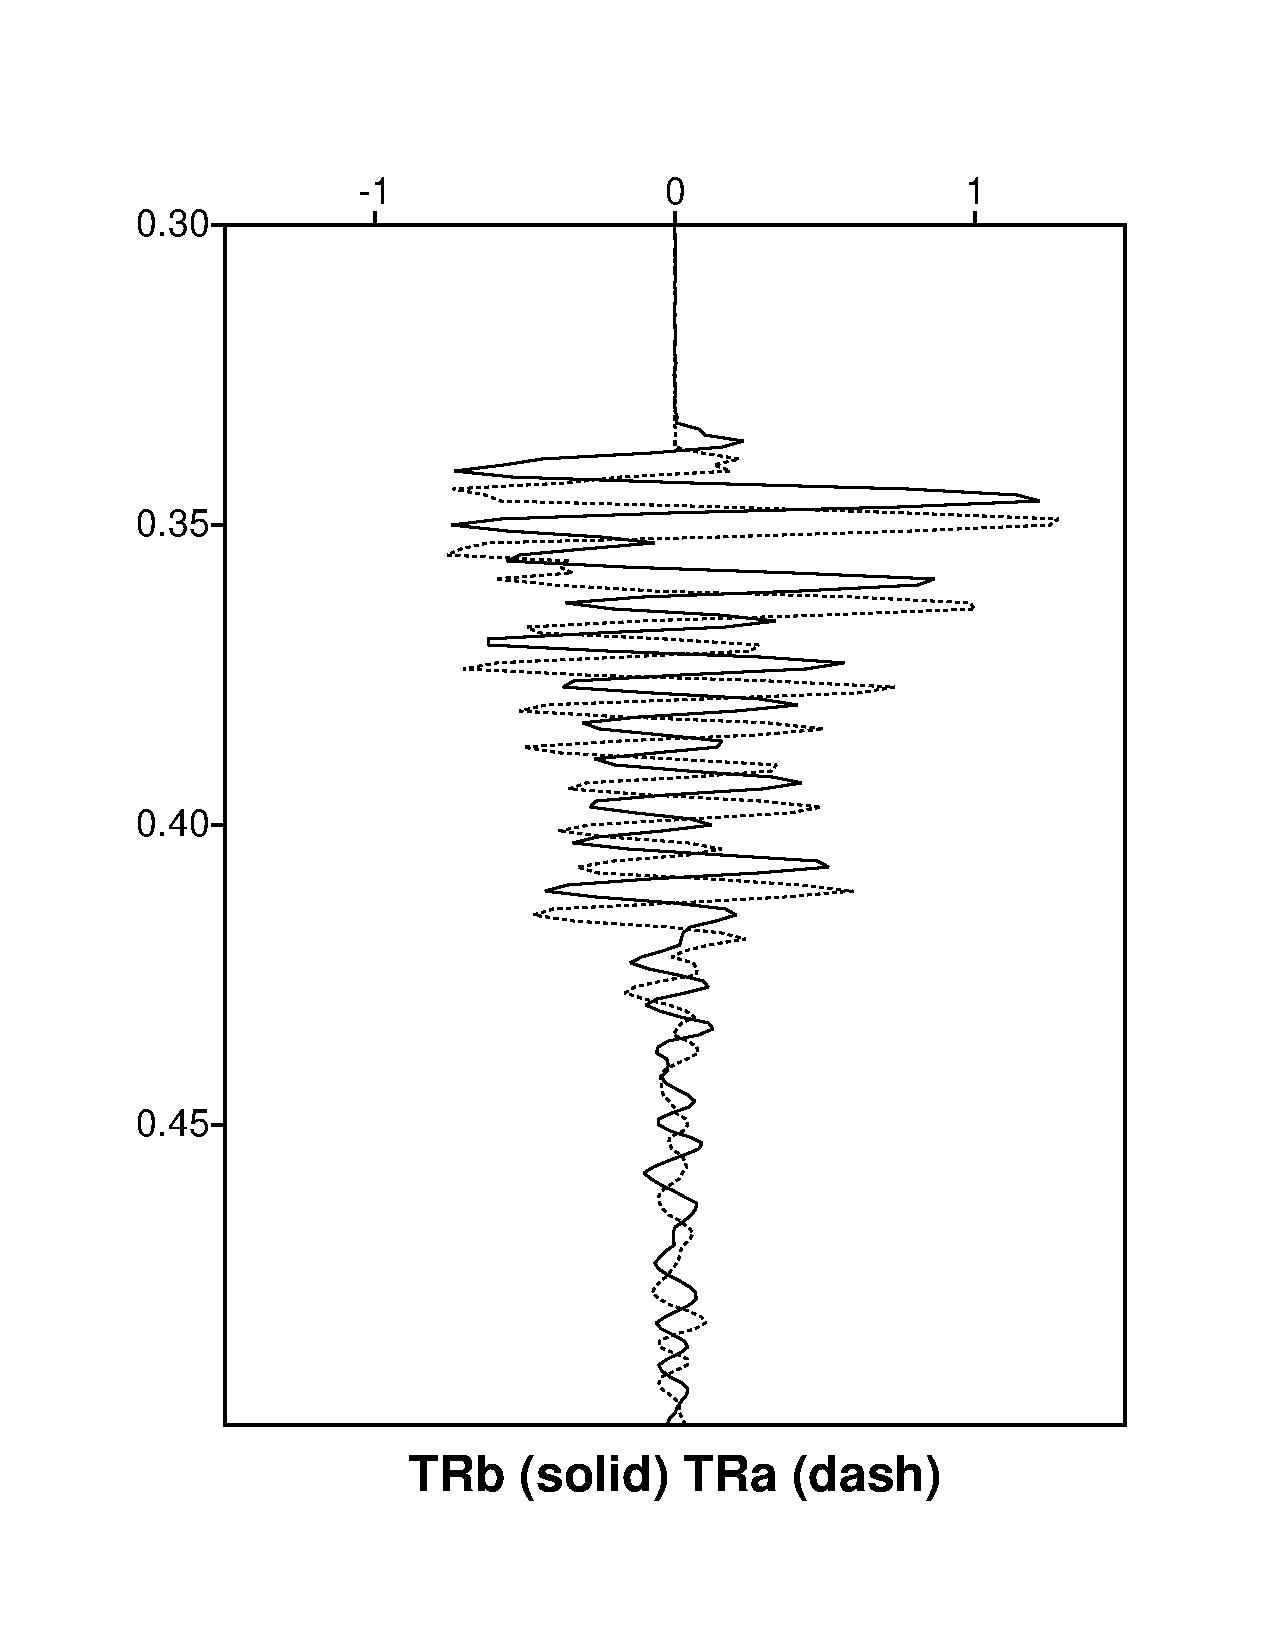
\includegraphics[width=0.45\textwidth]{Fig/fig1}}\\
%    \subfigure[]{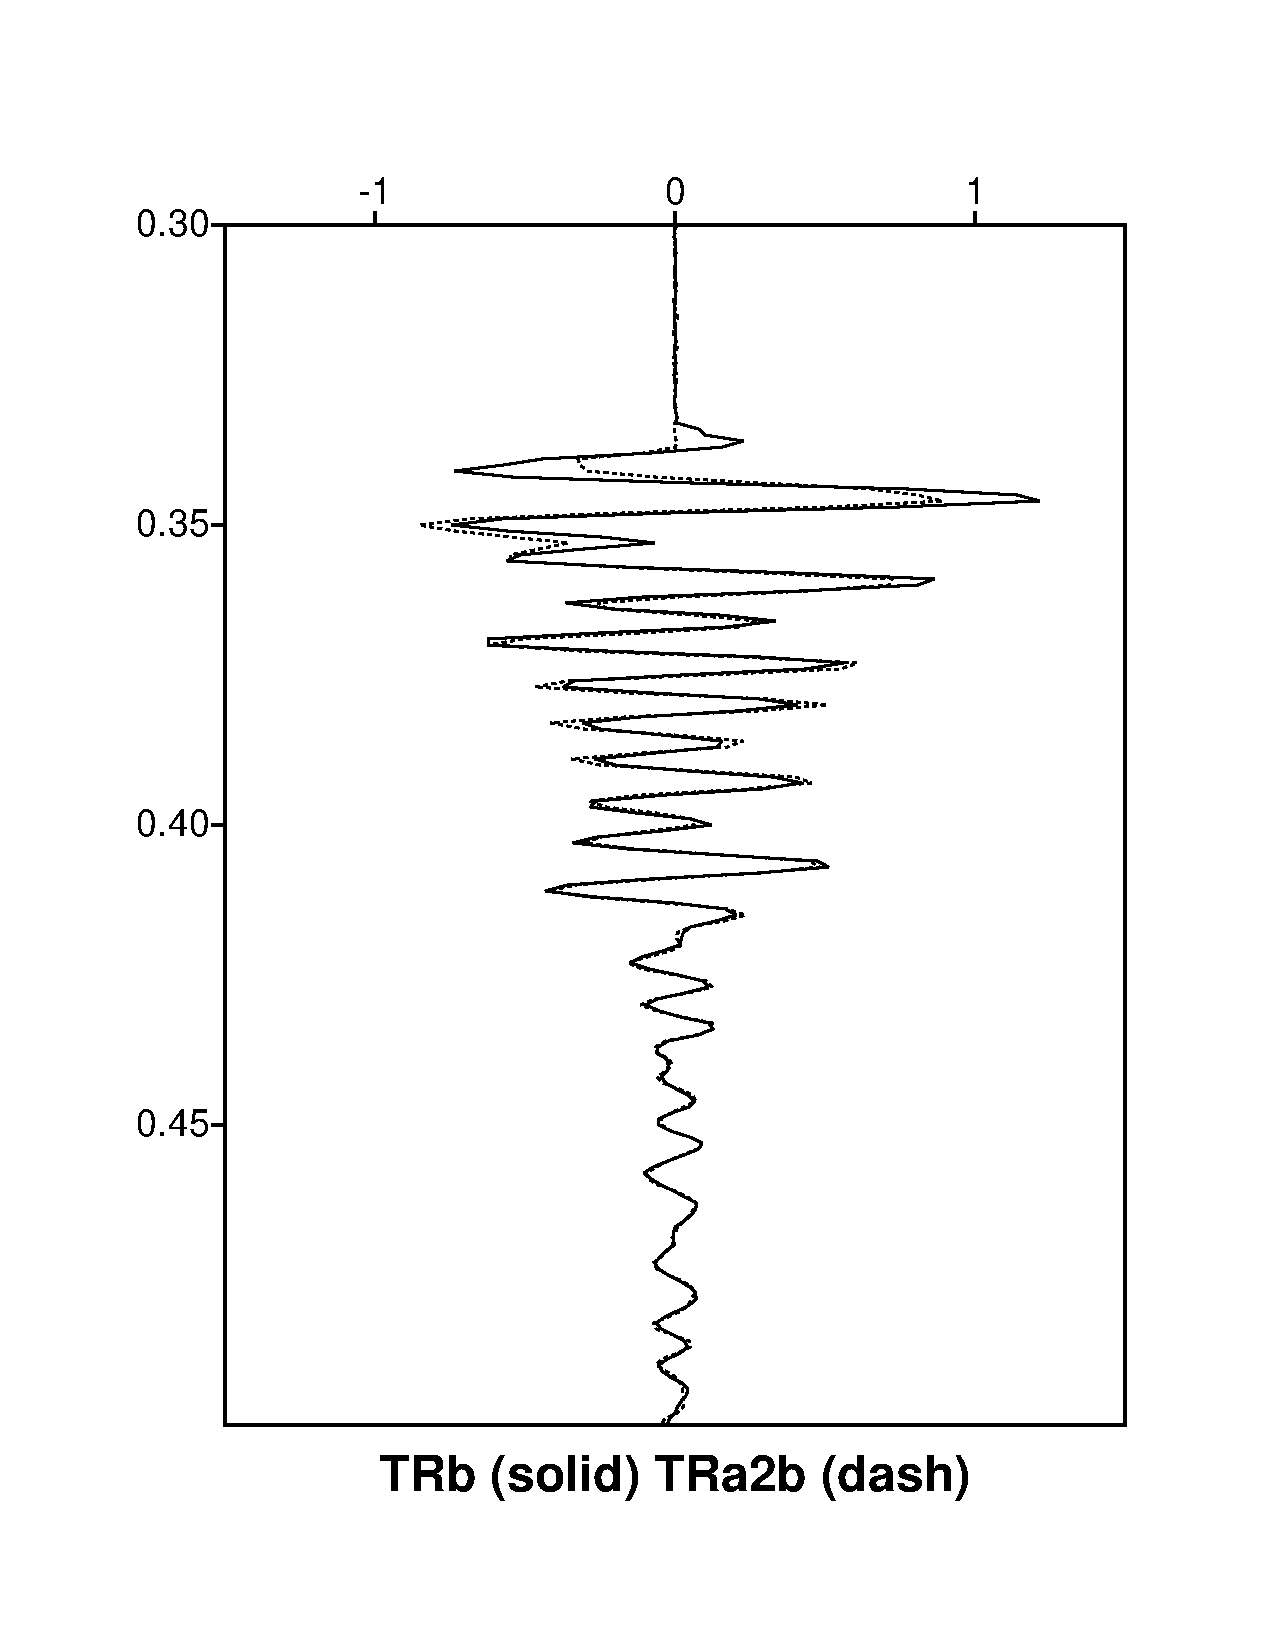
\includegraphics[width=0.45\textwidth]{Fig/fig2}}
%	\caption{(a) Caption a. (b) Caption b.}
%	\label{fig:fig1,fig2}
%\end{figure}

%\begin{table}[h]
%\caption{Table caption}
%\begin{center}
%     \begin{tabular}{|c|c|c|c|c|c|} 
%	  \hline Column1 (unit)  & Column2 (unit) & Column3 (unit) \\ 
%	  \hline 1 & 2  & 3 \\
%       \hline
%    \end{tabular} 
%\end{center}
%\label{tbl:table1}
%\end{table}





